\documentclass{article}
\usepackage{amsmath}
\usepackage{mathrsfs}
\usepackage{graphicx}
\usepackage{fontspec}
\setmainfont{Alegreya Sans SC}
% \setmainfont{AlegreyaSans-ExtraBoldItalic.otf}
% unicode-math should after fontspec
\usepackage{unicode-math}
\setmathfont{Latin Modern Math}




\begin{document}
\section{system fonts}
Lorem ipsum dolor sit amet, consectetuer adipiscing elit. Ut purus elit, vestibu-
lum ut, placerat ac, adipiscing vitae, felis. Curabitur dictum gravida mauris.
Nam arcu libero, nonumm

\textbf{Hello world}

Math calligraphic font:
\begin{align}
    % \mathcal{A} = \mathcal{B}+C 
    \mathscr{A} = \mathscr{B}+C    
\end{align}


TeX Gyre Pagella Math:
\setmathfont[range={\mathscr,\mathbfscr}]{TeX Gyre Pagella Math}
\begin{align}
    \mathscr{A} = \mathscr{B}+C    
\end{align}

TeX Gyre Termes Math:
\setmathfont[range={\mathscr,\mathbfscr}]{TeX Gyre Termes Math}
\begin{align}
    \mathscr{A} = \mathscr{B}+C    
\end{align}

TeX Gyre Bonum Math
\setmathfont[range={\mathscr,\mathbfscr}]{TeX Gyre Bonum Math}
\begin{align}
    \mathscr{A} = \mathscr{B}+C    
\end{align}

\begin{figure}[!htb]
    \centering
    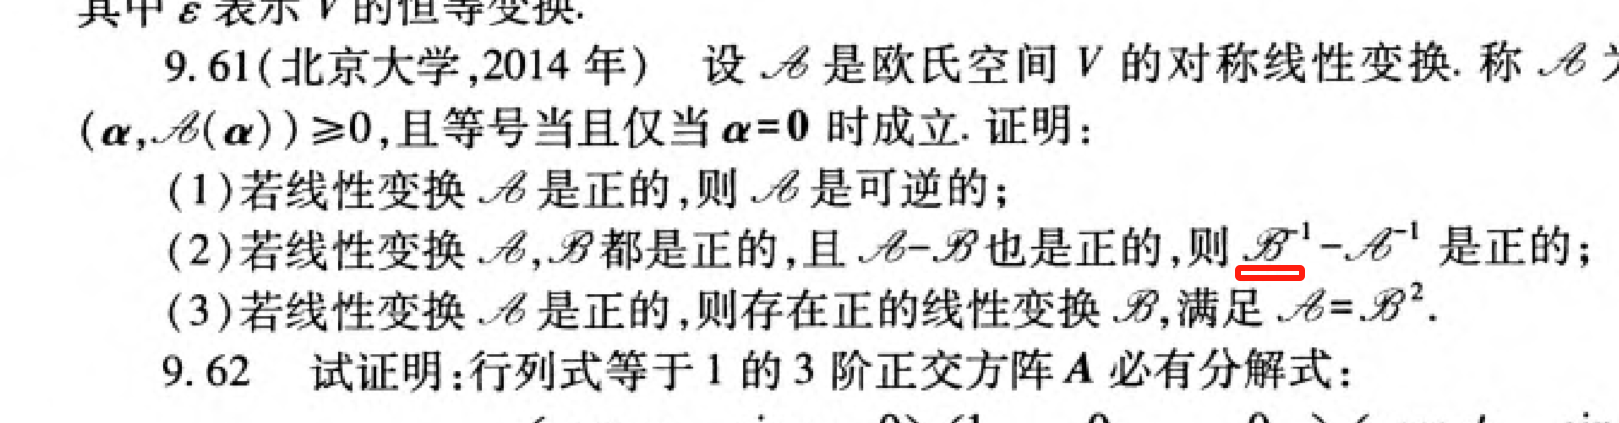
\includegraphics[width=.75\linewidth]{./example.png}
\end{figure}
\end{document}



